\section{Finite experiments}
\label{sec:experiments}

The experiments ask whether small-order closures reproduce the \emph{function
learned by dense gradient flow}.  They do not test only training labels.  Each
closure uses the same initialized weights as its dense reference and retains
the same $W_0$.  Unless stated otherwise, models are compared at their own
first crossing of the same training-loss target.  This is a matched-loss
endpoint comparison, not an equal-time comparison or a proof of continuous
time accuracy.

\subsection{Sparse-label functions on the circle}

The first panel uses bias-free two-hidden-layer tanh networks of width 2048,
canonical mobilities $(n,1,n)$, eight labeled unit-circle inputs, and one
initialization.  The equal-mixed task has an exact four-sample antipodal
quotient.  Dense and activity-clock trajectories stop at their own first
training-MSE $10^{-3}$ crossing.  Predictor discrepancy is RMS over 8192
equally spaced circle directions.

\begin{table}[t]
\centering
\small
\caption{Activity-clock RMS discrepancy from the dense fitted circle function.
Fresh dense references are used where available.  The two-outlier row retains
the study's selected archived reference.  The smallest P7 values are near or
below measured numerical-refinement sensitivity and should be read at their
order of magnitude.}
\label{tab:circle}
\begin{tabular}{@{}lrrr@{}}
\toprule
Task & $P=1$ & $P=3$ & $P=7$\\
\midrule
Two outliers, alternating & 0.236313 & 0.0729531 & 0.0046631\\
Quadrant, alternating & 0.341318 & 0.0456113 & 0.0015523\\
Quadrant, paired labels & 0.0192813 & 0.0028176 & 0.0001185\\
Quadrant, center/edges & 0.0455816 & 0.0048778 & 0.0013076\\
Equal mixed odd & 0.0123995 & 0.0005257 & $3.7\times10^{-6}$\\
\bottomrule
\end{tabular}
\end{table}

Figure~\ref{fig:circle-functions} shows the full learned functions.  The
training points occupy only a small part of the evaluation grid, so agreement
between curves is stronger evidence than common training fit.  There is no
ground-truth label function on the unlabeled circle; these are approximation
errors against dense learning, not generalization errors.

\begin{figure}[t]
\centering
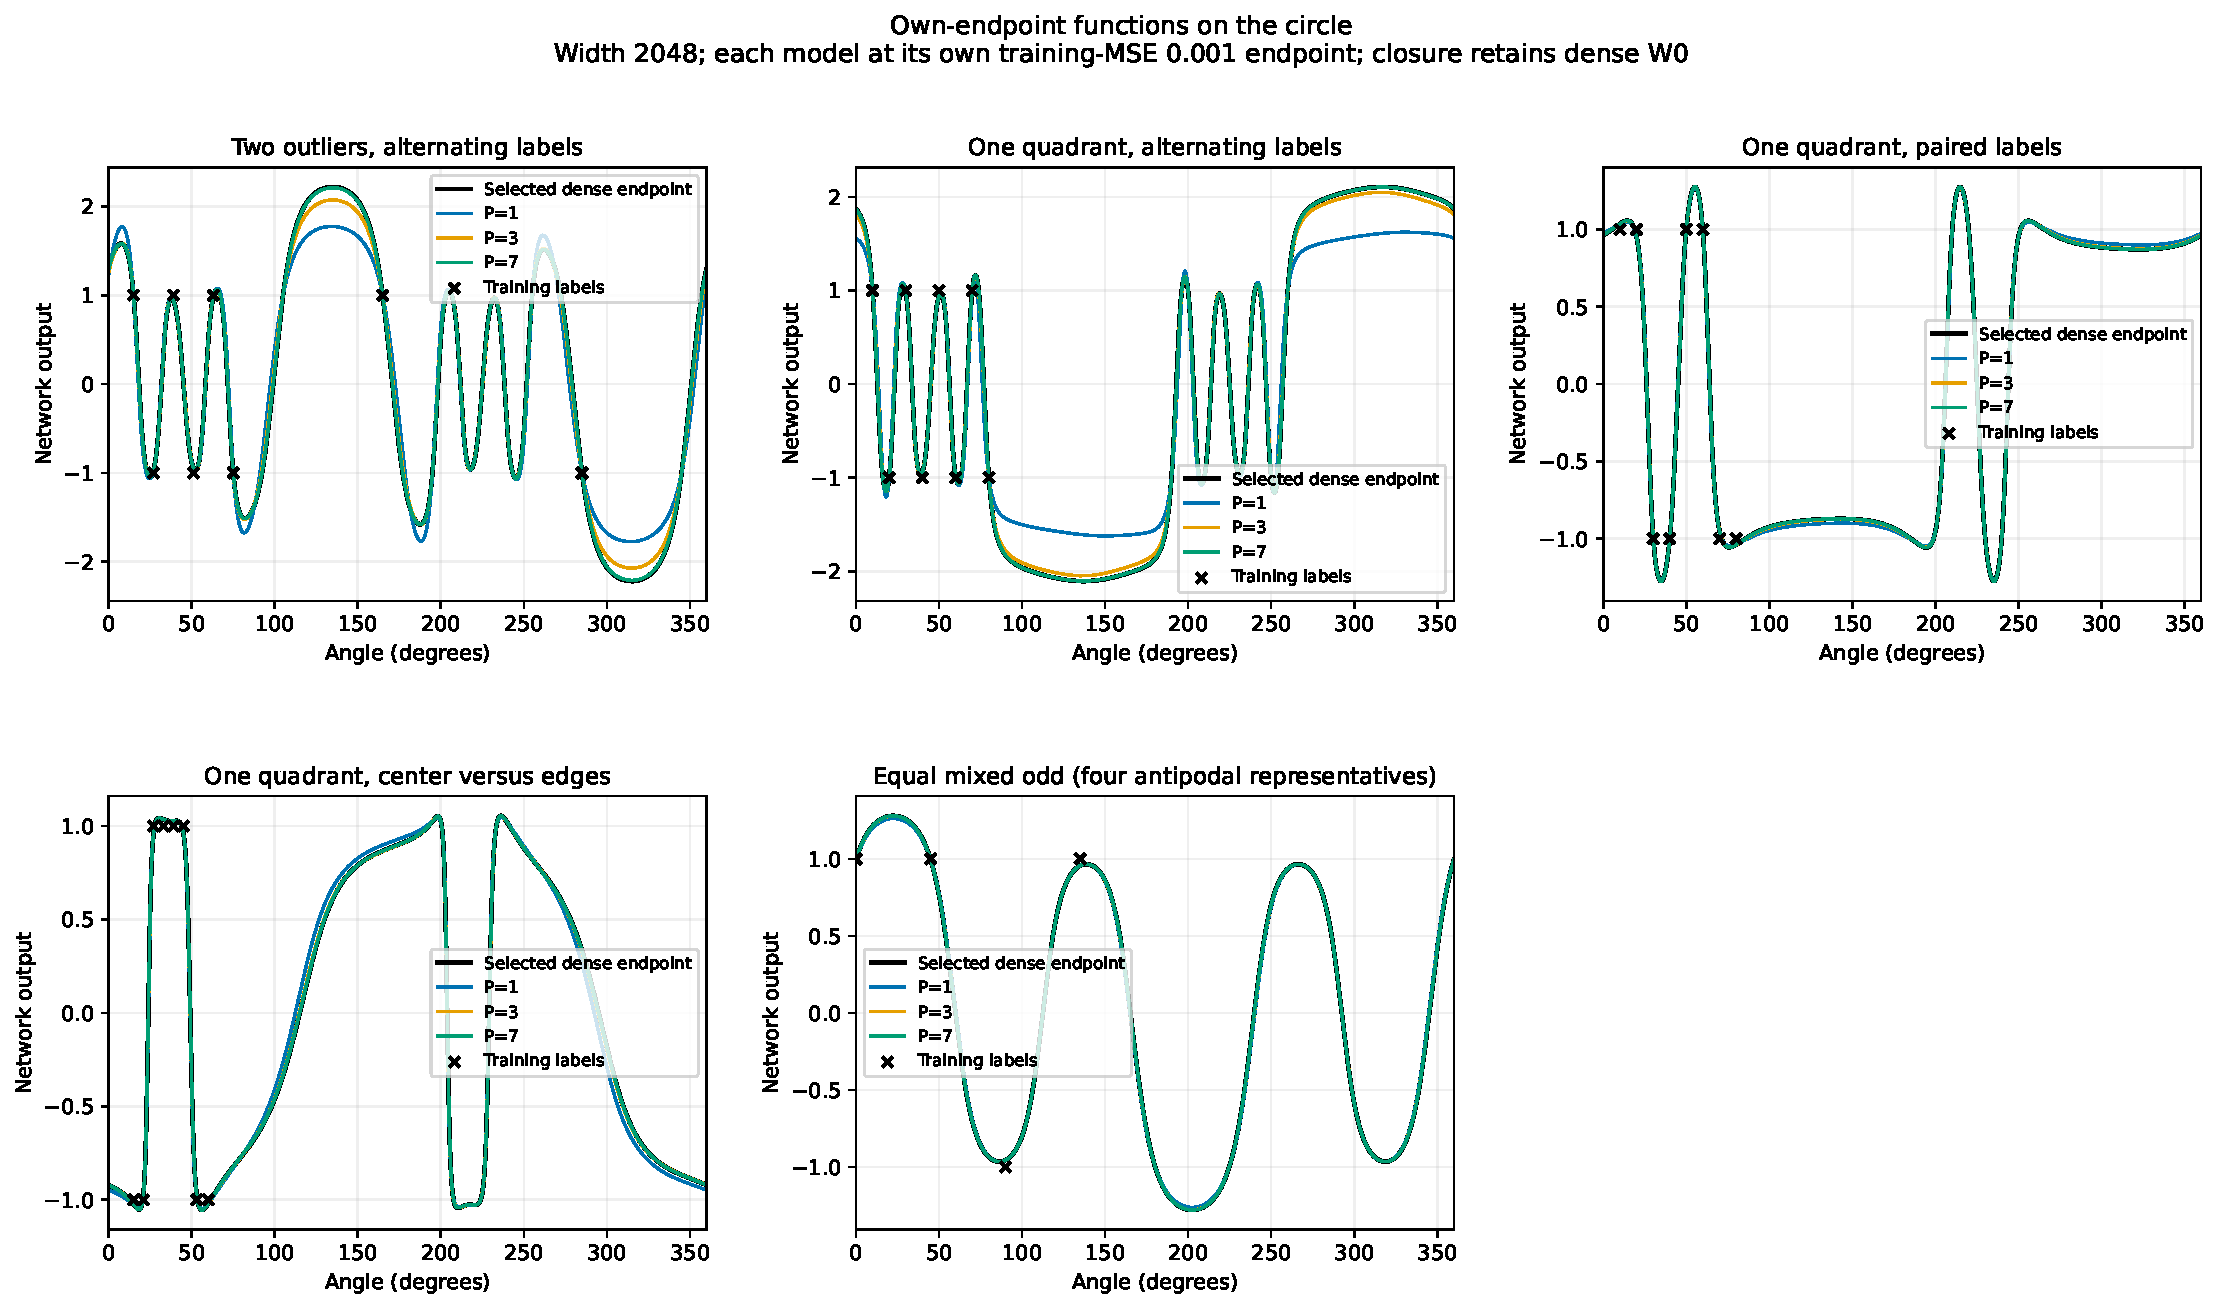
\includegraphics[width=\linewidth]{figures/circle_endpoint_functions.pdf}
\caption{Dense and activity-clock fitted functions for five circle tasks.
Every model is shown at its own first training-MSE $10^{-3}$ crossing.  The
closure retains the dense initialized middle matrix.  The hard-outlier dense
reference is inherited from the frozen benchmark; the other rows have fresh
references checked within the response-memory study.}
\label{fig:circle-functions}
\end{figure}

Figure~\ref{fig:circle-polar} gives the requested radial view for a fully
in-study fresh-reference task.  Network output is signed, so the plotted radius
is explicitly shifted by two; radial tick labels report the original output.

\begin{figure}[t]
\centering
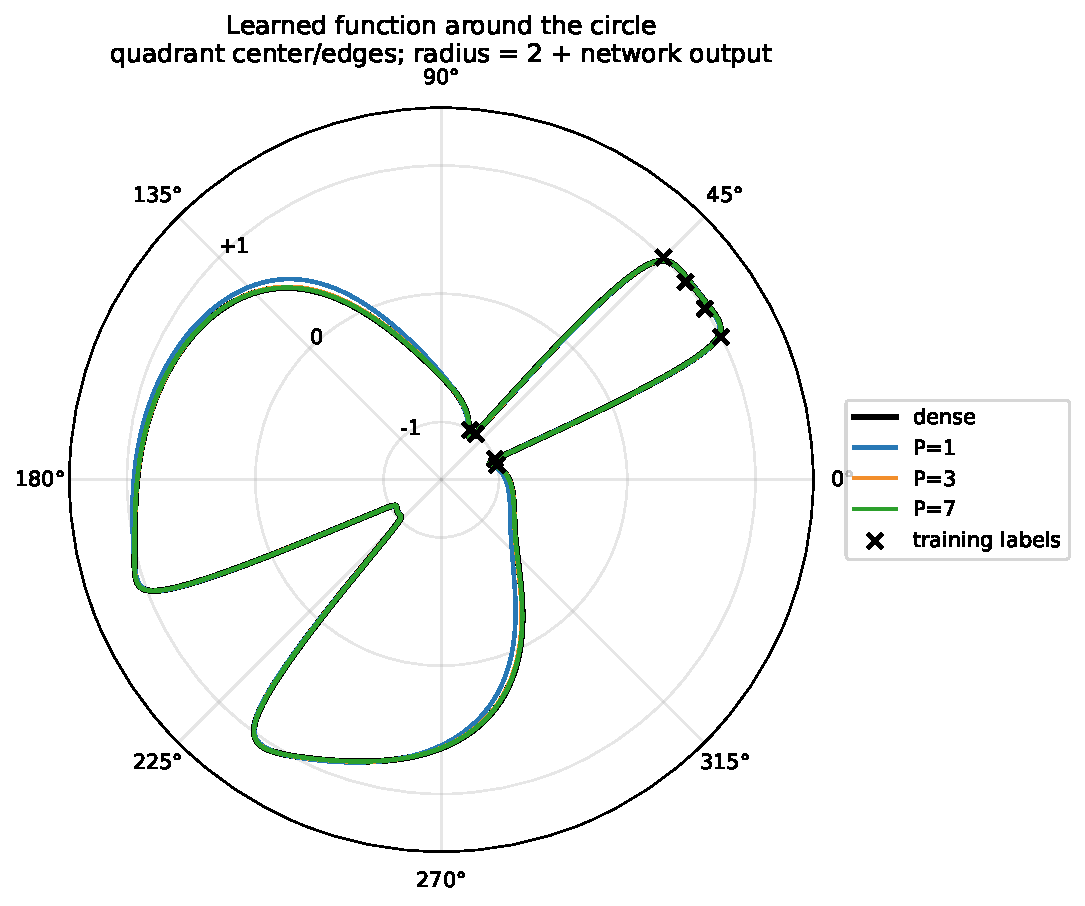
\includegraphics[width=0.72\linewidth]{figures/circle_polar_center_edges.pdf}
\caption{Polar rendering of the quadrant center/edges experiment.  The angle
is the input direction and radius is $2+f(x)$.  Black crosses are training
labels.  The figure is postprocessed from frozen predictions and involves no
new training.}
\label{fig:circle-polar}
\end{figure}

The same construction was tested with three hidden tanh layers of width 4096,
so two dense internal matrices were compressed simultaneously.  Every run
reached MSE $10^{-3}$ and passed the declared numerical gates.  Results in
Table~\ref{tab:deep-circle} show strong improvement over $P=1$, but also two
resolved $P=2$ versus $P=3$ reversals.

\begin{table}[t]
\centering
\small
\caption{Three-hidden-layer circle RMS discrepancy from dense learning at
matched MSE $10^{-3}$.}
\label{tab:deep-circle}
\begin{tabular}{@{}lrrr@{}}
\toprule
Task & $P=1$ & $P=2$ & $P=3$\\
\midrule
Two outliers, alternating & 0.108086 & \textbf{0.023797} & 0.031476\\
Quadrant, alternating & 0.274643 & \textbf{0.028358} & 0.058491\\
Quadrant, paired labels & 0.012186 & 0.003708 & \textbf{0.001215}\\
Quadrant, center/edges & 0.078973 & 0.025702 & \textbf{0.007246}\\
Equal mixed odd & 0.014985 & 0.002412 & \textbf{0.000282}\\
\bottomrule
\end{tabular}
\end{table}

\subsection{Evolving response memory versus fixed or directly trained factors}

The response moments are not a frozen dictionary.  Their columns change with
the current neural responses, and the reconstructed network feeds back into
their derivatives.  In the historical fixed-dictionary experiments, learned
increments were confined to spans chosen at initialization.  Such methods
could fit coefficients but could not acquire new response directions.  On the
same difficult circle functions they were much less efficient in the reported
vector counts.  Those counts do not match total storage because response
memory retains $W_0$.

A cleaner control inside the current study trains a direct factorization
$W=W_0+AB$ by its own Euclidean factor gradient flow, with matched correction
rank and two factor initializations.  Response memory has lower function RMS in
all 29 numerically valid paired cells; 28 differences exceed a factor of two.
At rank 24 on the alternating-outlier task, for example, $P=3$ response memory
has RMS $0.07295$, versus $0.46546$ and $0.46091$ for the two direct-factor
runs.  At rank 56, the response error is $0.00466$ versus $0.51621$ and
$0.25103$.  This rejects the explanation that any low-rank learned correction
would perform equally well under its natural factor flow.  It does not prove
optimality over all low-rank algorithms.

\begin{figure}[t]
\centering
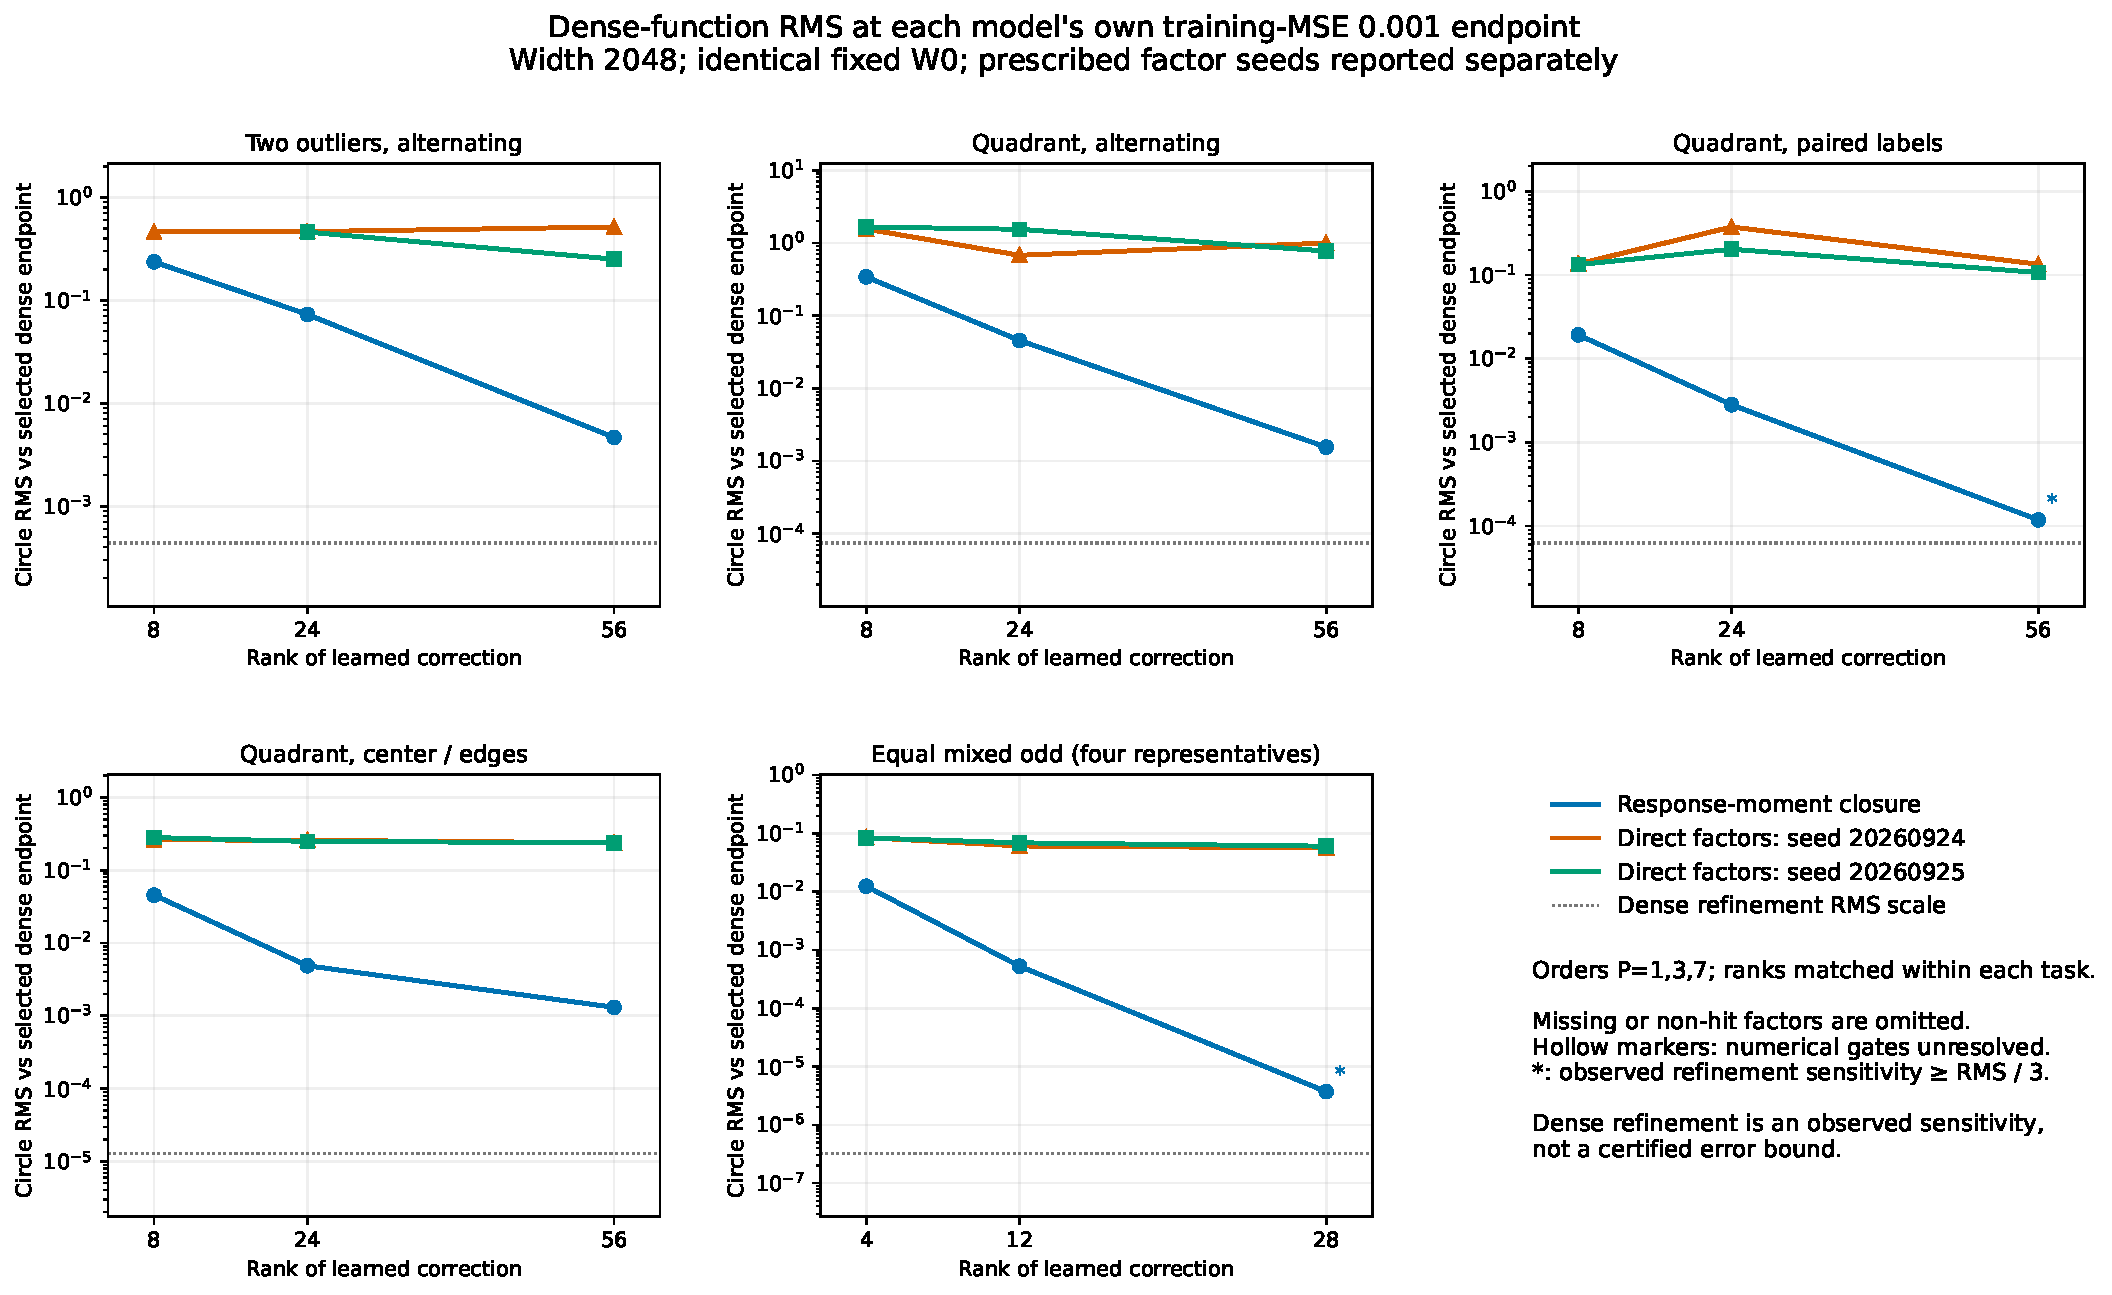
\includegraphics[width=0.88\linewidth]{figures/factor_rms_vs_rank.pdf}
\caption{Response-memory closure versus direct factor-gradient-flow controls
at matched structural rank.  Each model is compared with the same dense fitted
function.  Two factor seeds are shown; one capped factor cell is excluded from
fitted-endpoint comparison.}
\label{fig:factor-control}
\end{figure}

\subsection{MNIST predictions outside the training set}

The MNIST experiment uses digits 3 and 8, 50 training images per class, and all
1984 official-test images of those digits for evaluation.  Inputs are normalized
per image to unit Euclidean norm; no test image enters training, stopping, or
numerical control.  The network has two tanh hidden layers of width 4096.  At
each model's first training-MSE $10^{-3}$ crossing, held-out RMS discrepancy
from dense predictions is
\begin{equation}
 0.00324756\ (P=1),\qquad
 0.00108443\ (P=2),\qquad
 0.00119922\ (P=3).
\end{equation}
All declared refinement gates pass.  The small $P=3$ worsening relative to
$P=2$ is resolved under the frozen diagnostic rule.  All models have the same
held-out classification accuracy, but prediction agreement in
Figure~\ref{fig:mnist} is the relevant closure evidence.

\begin{figure}[t]
\centering
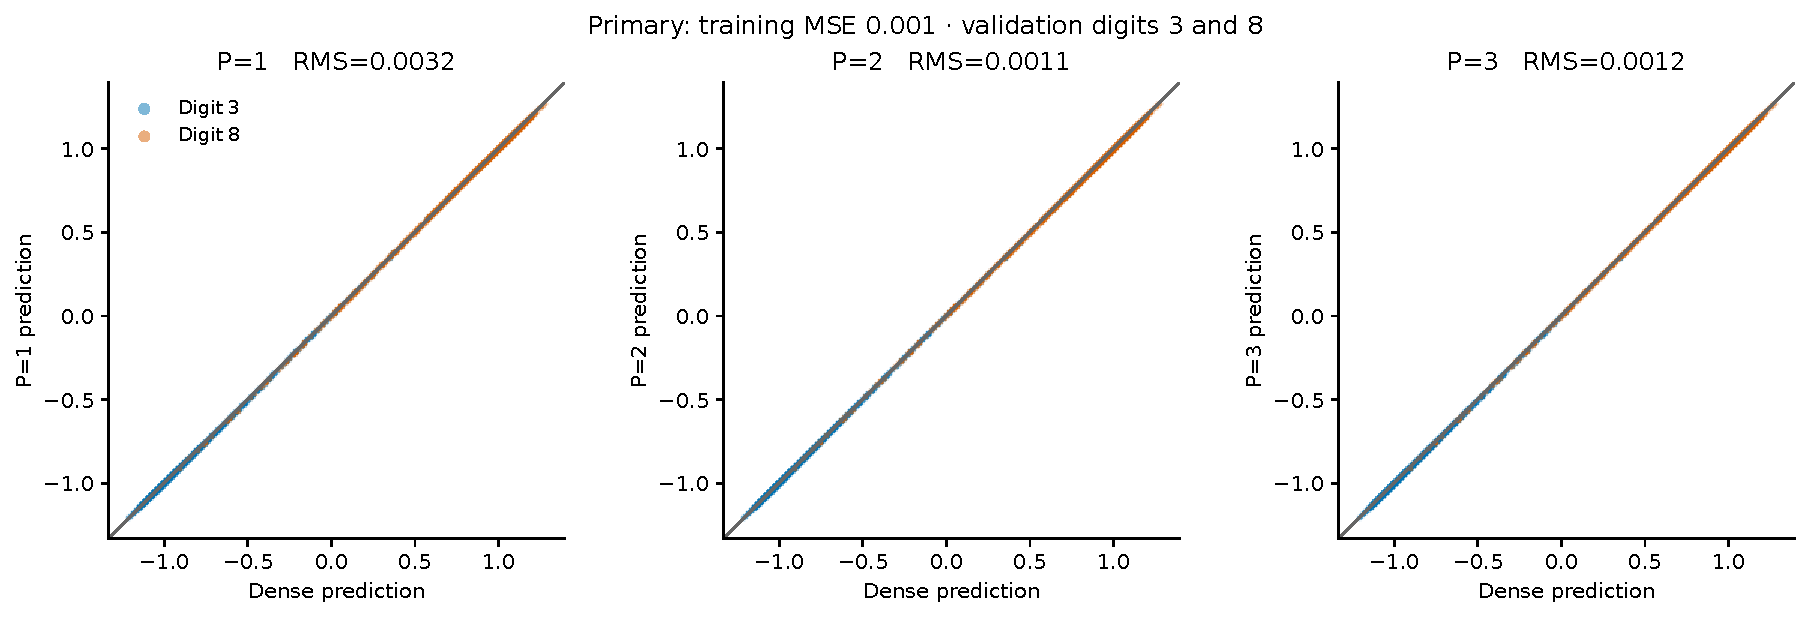
\includegraphics[width=\linewidth]{figures/mnist100_scatter.pdf}
\caption{Held-out closure predictions against dense predictions on 1984 MNIST
3/8 test images.  Models stop at their own training-MSE $10^{-3}$ endpoint.
The correction-rank bounds are 100, 200, and 300 for $P=1,2,3$.}
\label{fig:mnist}
\end{figure}

The history factors occupy $6.25$, $12.50$, and $18.75$ MiB, while an
unrestricted middle correction has $128$ MiB.  Adding the retained $128$ MiB
initialized matrix makes minimal total closure state slightly larger than the
dense current state.  Finest-tolerance integration took $103.0$ seconds for
dense flow and $139.9$, $149.9$, and $152.3$ seconds for the closures.  Measured
CUDA peaks were lower for the closures, but the experiment does not establish
a hardware-independent speedup.

\subsection{The sharper clock: promise and adverse cases}

The response clock has the stronger asymptotic theorem but need not dominate
at low order.  In a focused width-2048 fixed-step panel, all old- and new-clock
models reached training RMS $0.05$.  On the tanh alternating-quadrant task, the
new clock improves the $P=5$ full-circle discrepancy from $0.00658$ to
$0.00346$.  On GELU alternating outliers it improves old-clock $P=5$
$0.00196$ to $0.00098$.  On GELU alternating quadrant, however, its $P=5$
error is $0.99568$, versus $0.01279$ for the activity clock.  Halving the
maximum step reduces the new-clock error to $0.10313$, revealing substantial
finite-step sensitivity without eliminating the gap.

A broader single-seed response-clock sweep contains 82 activation/depth/task
configurations and 328 fits, each capped at 20 seconds.  Dense flow fits 79
configurations; $P=1,2,3$ fit 70, 67, and 66.  On the same 65 configurations
where all four models fit, median closure--dense test RMS is
$0.03147$, $0.01339$, and $0.00658$.  The largest fitted $P=3$ discrepancies
remain $1.36$, $1.25$, and $0.37$ on three alternating-quadrant cases.  The
panel supports typical improvement with order and documents clear exceptions.
It does not empirically verify an $O(P^{-2})$ rate.

All headline experiments use one initialization, and MNIST uses one selected
training subset.  Numerical refinement differences are sensitivity checks,
not rigorous error bars.  Appendix~\ref{app:experiment-tables} records the full
old/new-clock table and resource accounting used here.

